\title{Design Document: CS 378 Lab 2}
\author{Atharva Bendale (22B0901), Nivesh Aggarwal (22B0912), \\Dhvanil Gheewala (22B0923), Vishal Bysani (22B1061)}

\documentclass[11pt]{article}

\usepackage{amsmath}
\usepackage{amssymb}
\usepackage{hyperref}
\usepackage{ulem,graphicx}
\usepackage{subcaption}
\usepackage{gensymb}
\usepackage{tcolorbox}
\usepackage[margin=0.5in]{geometry}
\usepackage{tikz}
\usetikzlibrary{shapes.geometric, arrows}

\tikzstyle{startstop} = [ellipse, minimum width=1.5cm, minimum height=1cm, text centered, draw=black, fill=gray!30]
\tikzstyle{process} = [rectangle, minimum width=1.5cm, minimum height=1cm, text centered, draw=black, fill=orange!30]
\tikzstyle{decision} = [diamond, minimum width=1.5cm, minimum height=1cm, text centered, draw=black, fill=green!30]
\tikzstyle{arrow} = [thick,->,>=stealth]
\begin{document}
% \tcbset{
%   colframe=black,        % Frame color
%   colback=black!10!white, % Background color with transparency
%   boxrule=0.5mm,          % Thickness of the frame
%   arc=3mm,                % Round corners
%   outer arc=3mm,
%   boxsep=5mm,             % Space between the frame and the content
%   breakable,              % Allow breaking across pages
% }
\maketitle
\section{Encoding}
% Preamble, Manchester encoding, etc.
To ensure the proper reception of transmitted signal from the sender's device, we are using the following methods:
\begin{itemize}

    \item \textbf{Special Sequence}: We are using a special sequence of bits to mark the start of the message. This sequence is \texttt{000001}. When the reciever detects at leas 5 consecutive 0s, followed by a 1, it starts listening for the preamble. 
    \item \textbf{Preamble} : The preamble (5 bits) consists of the length of the original message encoded in binary. We then use a function \texttt{transmissionLength()} to get the length of the transmitted message after preamble, and receive the message accordingly. 
    \item \textbf{Return To Zero}: We are using the Return to Zero (RZ) encoding scheme to encode the bits. In this scheme, the signal returns to zero after each bit interval. This ensures that the receiver can easily detect the start and end of each bit. To encode a 0, we transmit a low frequency tone (1000 Hz) for half the bit duration and a middle frequency tone (2000 Hz) for the other half. For a 1, we transmit a high frequency tone (4000 Hz) for the first half and a middle frequency tone (2000 Hz) for the second half.  


\end{itemize}
\section{Error Detection}
To detect two bits of error in the transmitted message, our system uses a CRC-k algorithm with Hamming distance 5. In this algorithm we are using the polynomials under an assumption of low, constant bit error rate.
\begin{tcolorbox}[colback=black!10!white, colframe=black, title=Error Detection Algorithm ]
    \begin{verbatim}
1. Choose a CRC-k polynomial , where k is chosen according to the message length and use
the binary string of the polynomial as divisor
2. Append k 0s to the message and use this as the dividend and store the remainder as CRC 
code C(x) and send the xor of dividend and C(x)
3. When the modified message P(x) is received , our system uses binary polynomial division
with P(x) as dividend and C(x) as divisor. If the remainder is 0 it means that the P(x) is 
error free otherwise it has error\end{verbatim}
\end{tcolorbox}
To further optimise this procedure, we are using different degree polynomials for reducing the length of transmission as the length is variable. This information is shared with the receiver through the help of the preamble which has the length encoded in it. \\
All the chosen polynomials have the property that each remainder is mapped to a single transmitted message which has its atmost two bits altered. This property makes the polynomials special and ensures the correctness of our algorithm.
\section{Error Correction}
If our system detects any error using the error detection algorithm, we iterate over all possible pairs of indices , flip those bits and use the subroutine of error detection algorithms to check whether the current mutated message is error free or not. This method ensures not to find another correct code word because we have chosen a Hamming Distance of 5, and even if it ends up flipping 2 wrong bits (4 flipped in total along with the original error bits) it will not end up at another correct code word.  Since the length of the original message is upto 20 bits and the transmitted message can be upto 30 bits, the computation of \( \binom{30}{2} \) can be done quickly. The flowchart of the above procedure : 
\begin{center}
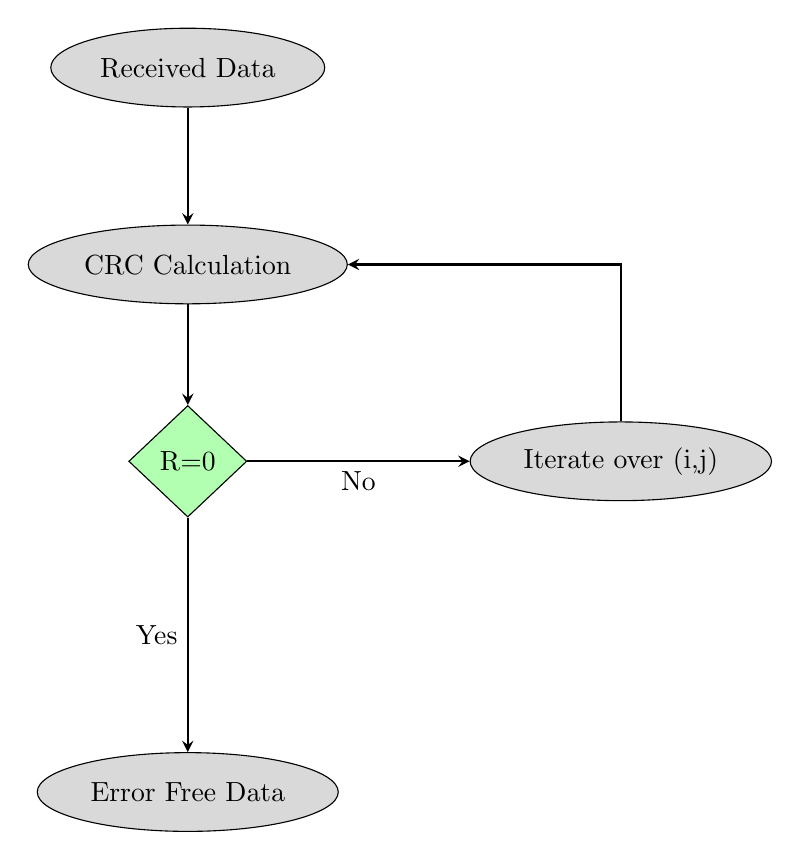
\begin{tikzpicture}[node distance=2.5cm] % Adjust node distance for better spacing

% Nodes
\node (received) [startstop] {Received Data};
\node (crc) [startstop, below of=received] {CRC Calculation};
\node (decision) [decision, below of=crc] {R=0};
\node (errorfree) [startstop, below of=decision, yshift=-1.7cm] {Error Free Data};
\node (ij) [startstop, right of=decision, xshift=3cm]{Iterate over (i,j)};

% Arrows
\draw [arrow] (received) -- (crc);
\draw [arrow] (crc) -- (decision);
\draw [arrow] (decision) -- node[anchor=east] {Yes} (errorfree);
\draw [arrow] (decision) -- node[anchor=north] {No} (ij);
\draw [arrow] (ij) |- (crc);

\end{tikzpicture}
\end{center}
\section{Reception}

The reception process in our system focuses on accurately converting the transmitted audio signal back into the original binary sequence. This involves a series of signal processing steps designed to handle noise, detect frequency tones, and decode them into bits. Below, we describe the major components of the reception pipeline.

\subsection{Audio Reception}
The audio signal is captured using the \texttt{receive\_audio()} function, which utilizes the PyAudio library. The system is configured with a sample rate of 44.1 kHz and collects data over a specified duration. We divide the audio stream into frames, with each frame containing 1024 samples. These frames are stored and then concatenated to form the full audio signal as a NumPy array for further processing.
\begin{tcolorbox}[colback=black!10!white, colframe=black]
\begin{verbatim}
audio = pyaudio.PyAudio()
stream = audio.open(format=pyaudio.paFloat32, channels=1, rate=sample_rate, input=True, 
                    frames_per_buffer=1024)
for _ in range(0, int(sample_rate / 1024 * duration)): 
    data = stream.read(1024) 
    frames.append(data)
\end{verbatim}
\end{tcolorbox}
\subsection{Noise Reduction}
To mitigate noise, we run the \texttt{calibrate} function to determine the average noise level in various frequency ranges of the received audio signal. We then use this information to filter out noise from the audio signal by subtracting the average noise level from the signal's power spectrum. This process helps improve the accuracy of frequency detection and bit decoding.
\begin{tcolorbox}[colback=black!10!white, colframe=black]
\begin{verbatim}
for _ in range(0, segment_size*white_noise_sample_size, segment_size):
  segment = self.receive_audio(stream, bit_duration, sample_rate)
  freqs, power = signal.welch(segment, sample_rate)
  low_freq_power = np.sum(power[(freqs >= self.low_freq-100) & 
                                                    (freqs <= self.low_freq+100)])
    mid_freq_power = np.sum(power[(freqs >= self.mid_freq-100) & 
                                                    (freqs <= self.mid_freq+100)])
    high_freq_power = np.sum(power[(freqs >= self.high_freq-100) & 
                                                    (freqs <= self.high_freq+100)])

    self.low_noise_avg += low_freq_power
    self.high_noise_avg += high_freq_power
    self.mid_noise_avg += mid_freq_power

self.low_noise_avg = self.low_noise_avg / white_noise_sample_size
self.high_noise_avg = self.high_noise_avg / white_noise_sample_size
self.mid_noise_avg = self.mid_noise_avg / white_noise_sample_size

\end{verbatim}
\end{tcolorbox}

\subsection{Frequency-Based Decoding}

The core of the reception mechanism involves detecting the frequency components of the received audio signal to determine the transmitted bits. Each bit is encoded as a specific frequency tone (1000 Hz for bit 0 and 3000 Hz for bit 1). After segmenting the audio signal into smaller chunks corresponding to each bit's duration, we analyze the frequency content of each segment (received using PyAudio) by applying Welch's method, implemented using the \texttt{signal} library from SciPy, for estimating power spectral density.
\begin{tcolorbox}[colback=black!10!white, colframe=black]
    
\begin{verbatim} 
freqs, power = signal.welch(segment, sample_rate) 
low_freq_power = np.sum(power[(freqs >= 900) & (freqs <= 1100)])
high_freq_power = np.sum(power[(freqs >= 2900) & (freqs <= 3100)])

if low_freq_power > high_freq_power: 
    bits.append(0) 
else: 
    bits.append(1) \end{verbatim}
\end{tcolorbox}

By summing the power within predefined frequency ranges, we can classify each segment as either a 0 or a 1 depending on which frequency range exhibits higher power. This method improves the robustness of frequency detection compared to simply using the Fast Fourier Transform (FFT), as it better handles noisy signals and overlapping frequencies.

\subsection{Message Beginning Detection}
To accurately detect the start of a transmitted message, we introduce a preamble system. A predefined special subsequence \texttt{01111110} is being sent continuously initially. When this subsequence ends, the receiver starts listening for the preamble (consisting of the length of the message which follows). The receiver then listens to the message and employs the error-detection and error-correction mechanism as described above.

\section{Citations}
% \begin{tcolorbox}
The polynomials used in our systems are obtained from: \href{https://users.ece.cmu.edu/~koopman/crc/hd5.html}{Best CRC Polynomials}.
% \end{tcolorbox}
\end{document}